\documentclass[10pt,a4paper,onecolumn]{article}
\usepackage{marginnote}
\usepackage{graphicx}
\usepackage{xcolor}
\usepackage{authblk,etoolbox}
\usepackage{titlesec}
\usepackage{calc}
\usepackage{tikz}
\usepackage{hyperref}
\hypersetup{colorlinks,breaklinks,
            urlcolor=[rgb]{0.0, 0.5, 1.0},
            linkcolor=[rgb]{0.0, 0.5, 1.0}}
\usepackage{caption}
\usepackage{tcolorbox}
\usepackage{amssymb,amsmath}
\usepackage{ifxetex,ifluatex}
\usepackage{seqsplit}
\usepackage{fixltx2e} % provides \textsubscript
\usepackage[
  backend=biber,
%  style=alphabetic,
%  citestyle=numeric
]{biblatex}
\bibliography{paper.bib}



% --- Page layout -------------------------------------------------------------
\usepackage[top=3.5cm, bottom=3cm, right=1.5cm, left=1.0cm,
            headheight=2.2cm, reversemp, includemp, marginparwidth=4.5cm]{geometry}

% --- Default font ------------------------------------------------------------
% \renewcommand\familydefault{\sfdefault}

% --- Style -------------------------------------------------------------------
\renewcommand{\bibfont}{\small \sffamily}
\renewcommand{\captionfont}{\small\sffamily}
\renewcommand{\captionlabelfont}{\bfseries}

% --- Section/SubSection/SubSubSection ----------------------------------------
\titleformat{\section}
  {\normalfont\sffamily\Large\bfseries}
  {}{0pt}{}
\titleformat{\subsection}
  {\normalfont\sffamily\large\bfseries}
  {}{0pt}{}
\titleformat{\subsubsection}
  {\normalfont\sffamily\bfseries}
  {}{0pt}{}
\titleformat*{\paragraph}
  {\sffamily\normalsize}


% --- Header / Footer ---------------------------------------------------------
\usepackage{fancyhdr}
\pagestyle{fancy}
\fancyhf{}
%\renewcommand{\headrulewidth}{0.50pt}
\renewcommand{\headrulewidth}{0pt}
\fancyhead[L]{\hspace{-0.75cm}\includegraphics[width=5.5cm]{C:/Users/ben29/AppData/Local/R/win-library/4.2/rticles/rmarkdown/templates/joss/resources/JOSS-logo.png}}
\fancyhead[C]{}
\fancyhead[R]{}
\renewcommand{\footrulewidth}{0.25pt}

\fancyfoot[L]{\footnotesize{\sffamily , (). ig.degree.betweenness: A
Community Detection Algorithm Leveraging Degree
Centrality. \textit{Journal of Open Source Software}, (), . \href{https://doi.org/}{https://doi.org/}}}


\fancyfoot[R]{\sffamily \thepage}
\makeatletter
\let\ps@plain\ps@fancy
\fancyheadoffset[L]{4.5cm}
\fancyfootoffset[L]{4.5cm}

% --- Macros ---------

\definecolor{linky}{rgb}{0.0, 0.5, 1.0}

\newtcolorbox{repobox}
   {colback=red, colframe=red!75!black,
     boxrule=0.5pt, arc=2pt, left=6pt, right=6pt, top=3pt, bottom=3pt}

\newcommand{\ExternalLink}{%
   \tikz[x=1.2ex, y=1.2ex, baseline=-0.05ex]{%
       \begin{scope}[x=1ex, y=1ex]
           \clip (-0.1,-0.1)
               --++ (-0, 1.2)
               --++ (0.6, 0)
               --++ (0, -0.6)
               --++ (0.6, 0)
               --++ (0, -1);
           \path[draw,
               line width = 0.5,
               rounded corners=0.5]
               (0,0) rectangle (1,1);
       \end{scope}
       \path[draw, line width = 0.5] (0.5, 0.5)
           -- (1, 1);
       \path[draw, line width = 0.5] (0.6, 1)
           -- (1, 1) -- (1, 0.6);
       }
   }

% --- Title / Authors ---------------------------------------------------------
% patch \maketitle so that it doesn't center
\patchcmd{\@maketitle}{center}{flushleft}{}{}
\patchcmd{\@maketitle}{center}{flushleft}{}{}
% patch \maketitle so that the font size for the title is normal
\patchcmd{\@maketitle}{\LARGE}{\LARGE\sffamily}{}{}
% patch the patch by authblk so that the author block is flush left
\def\maketitle{{%
  \renewenvironment{tabular}[2][]
    {\begin{flushleft}}
    {\end{flushleft}}
  \AB@maketitle}}
\makeatletter
\renewcommand\AB@affilsepx{ \protect\Affilfont}
%\renewcommand\AB@affilnote[1]{{\bfseries #1}\hspace{2pt}}
\renewcommand\AB@affilnote[1]{{\bfseries #1}\hspace{3pt}}
\makeatother
\renewcommand\Authfont{\sffamily\bfseries}
\renewcommand\Affilfont{\sffamily\small\mdseries}
\setlength{\affilsep}{1em}


\ifnum 0\ifxetex 1\fi\ifluatex 1\fi=0 % if pdftex
  \usepackage[T1]{fontenc}
  \usepackage[utf8]{inputenc}

\else % if luatex or xelatex
  \ifxetex
    \usepackage{mathspec}
  \else
    \usepackage{fontspec}
  \fi
  \defaultfontfeatures{Ligatures=TeX,Scale=MatchLowercase}

\fi
% use upquote if available, for straight quotes in verbatim environments
\IfFileExists{upquote.sty}{\usepackage{upquote}}{}
% use microtype if available
\IfFileExists{microtype.sty}{%
\usepackage{microtype}
\UseMicrotypeSet[protrusion]{basicmath} % disable protrusion for tt fonts
}{}

\usepackage{hyperref}
\hypersetup{unicode=true,
            pdftitle={ig.degree.betweenness: A Community Detection Algorithm Leveraging Degree Centrality},
            pdfauthor={Benjamin Smith},
            pdfborder={0 0 0},
            breaklinks=true}
\urlstyle{same}  % don't use monospace font for urls
\usepackage{graphicx,grffile}
\makeatletter
\def\maxwidth{\ifdim\Gin@nat@width>\linewidth\linewidth\else\Gin@nat@width\fi}
\def\maxheight{\ifdim\Gin@nat@height>\textheight\textheight\else\Gin@nat@height\fi}
\makeatother
% Scale images if necessary, so that they will not overflow the page
% margins by default, and it is still possible to overwrite the defaults
% using explicit options in \includegraphics[width, height, ...]{}
\setkeys{Gin}{width=\maxwidth,height=\maxheight,keepaspectratio}
\IfFileExists{parskip.sty}{%
\usepackage{parskip}
}{% else
\setlength{\parindent}{0pt}
\setlength{\parskip}{6pt plus 2pt minus 1pt}
}
\setlength{\emergencystretch}{3em}  % prevent overfull lines
\setcounter{secnumdepth}{0}
% Redefines (sub)paragraphs to behave more like sections
\ifx\paragraph\undefined\else
\let\oldparagraph\paragraph
\renewcommand{\paragraph}[1]{\oldparagraph{#1}\mbox{}}
\fi
\ifx\subparagraph\undefined\else
\let\oldsubparagraph\subparagraph
\renewcommand{\subparagraph}[1]{\oldsubparagraph{#1}\mbox{}}
\fi

% Pandoc syntax highlighting
\usepackage{color}
\usepackage{fancyvrb}
\newcommand{\VerbBar}{|}
\newcommand{\VERB}{\Verb[commandchars=\\\{\}]}
\DefineVerbatimEnvironment{Highlighting}{Verbatim}{commandchars=\\\{\}}
% Add ',fontsize=\small' for more characters per line
\usepackage{framed}
\definecolor{shadecolor}{RGB}{248,248,248}
\newenvironment{Shaded}{\begin{snugshade}}{\end{snugshade}}
\newcommand{\AlertTok}[1]{\textcolor[rgb]{0.94,0.16,0.16}{#1}}
\newcommand{\AnnotationTok}[1]{\textcolor[rgb]{0.56,0.35,0.01}{\textbf{\textit{#1}}}}
\newcommand{\AttributeTok}[1]{\textcolor[rgb]{0.13,0.29,0.53}{#1}}
\newcommand{\BaseNTok}[1]{\textcolor[rgb]{0.00,0.00,0.81}{#1}}
\newcommand{\BuiltInTok}[1]{#1}
\newcommand{\CharTok}[1]{\textcolor[rgb]{0.31,0.60,0.02}{#1}}
\newcommand{\CommentTok}[1]{\textcolor[rgb]{0.56,0.35,0.01}{\textit{#1}}}
\newcommand{\CommentVarTok}[1]{\textcolor[rgb]{0.56,0.35,0.01}{\textbf{\textit{#1}}}}
\newcommand{\ConstantTok}[1]{\textcolor[rgb]{0.56,0.35,0.01}{#1}}
\newcommand{\ControlFlowTok}[1]{\textcolor[rgb]{0.13,0.29,0.53}{\textbf{#1}}}
\newcommand{\DataTypeTok}[1]{\textcolor[rgb]{0.13,0.29,0.53}{#1}}
\newcommand{\DecValTok}[1]{\textcolor[rgb]{0.00,0.00,0.81}{#1}}
\newcommand{\DocumentationTok}[1]{\textcolor[rgb]{0.56,0.35,0.01}{\textbf{\textit{#1}}}}
\newcommand{\ErrorTok}[1]{\textcolor[rgb]{0.64,0.00,0.00}{\textbf{#1}}}
\newcommand{\ExtensionTok}[1]{#1}
\newcommand{\FloatTok}[1]{\textcolor[rgb]{0.00,0.00,0.81}{#1}}
\newcommand{\FunctionTok}[1]{\textcolor[rgb]{0.13,0.29,0.53}{\textbf{#1}}}
\newcommand{\ImportTok}[1]{#1}
\newcommand{\InformationTok}[1]{\textcolor[rgb]{0.56,0.35,0.01}{\textbf{\textit{#1}}}}
\newcommand{\KeywordTok}[1]{\textcolor[rgb]{0.13,0.29,0.53}{\textbf{#1}}}
\newcommand{\NormalTok}[1]{#1}
\newcommand{\OperatorTok}[1]{\textcolor[rgb]{0.81,0.36,0.00}{\textbf{#1}}}
\newcommand{\OtherTok}[1]{\textcolor[rgb]{0.56,0.35,0.01}{#1}}
\newcommand{\PreprocessorTok}[1]{\textcolor[rgb]{0.56,0.35,0.01}{\textit{#1}}}
\newcommand{\RegionMarkerTok}[1]{#1}
\newcommand{\SpecialCharTok}[1]{\textcolor[rgb]{0.81,0.36,0.00}{\textbf{#1}}}
\newcommand{\SpecialStringTok}[1]{\textcolor[rgb]{0.31,0.60,0.02}{#1}}
\newcommand{\StringTok}[1]{\textcolor[rgb]{0.31,0.60,0.02}{#1}}
\newcommand{\VariableTok}[1]{\textcolor[rgb]{0.00,0.00,0.00}{#1}}
\newcommand{\VerbatimStringTok}[1]{\textcolor[rgb]{0.31,0.60,0.02}{#1}}
\newcommand{\WarningTok}[1]{\textcolor[rgb]{0.56,0.35,0.01}{\textbf{\textit{#1}}}}

% tightlist command for lists without linebreak
\providecommand{\tightlist}{%
  \setlength{\itemsep}{0pt}\setlength{\parskip}{0pt}}


% Pandoc citation processing
%From Pandoc 3.1.8
% definitions for citeproc citations
\NewDocumentCommand\citeproctext{}{}
\NewDocumentCommand\citeproc{mm}{%
  \begingroup\def\citeproctext{#2}\cite{#1}\endgroup}
\makeatletter
 % allow citations to break across lines
 \let\@cite@ofmt\@firstofone
 % avoid brackets around text for \cite:
 \def\@biblabel#1{}
 \def\@cite#1#2{{#1\if@tempswa , #2\fi}}
\makeatother
\newlength{\cslhangindent}
\setlength{\cslhangindent}{1.5em}
\newlength{\csllabelwidth}
\setlength{\csllabelwidth}{3em}
\newenvironment{CSLReferences}[2] % #1 hanging-indent, #2 entry-spacing
 {\begin{list}{}{%
  \setlength{\itemindent}{0pt}
  \setlength{\leftmargin}{0pt}
  \setlength{\parsep}{0pt}
  % turn on hanging indent if param 1 is 1
  \ifodd #1
   \setlength{\leftmargin}{\cslhangindent}
   \setlength{\itemindent}{-1\cslhangindent}
  \fi
  % set entry spacing
  \setlength{\itemsep}{#2\baselineskip}}}
 {\end{list}}
\usepackage{calc}
\newcommand{\CSLBlock}[1]{#1\hfill\break}
\newcommand{\CSLLeftMargin}[1]{\parbox[t]{\csllabelwidth}{#1}}
\newcommand{\CSLRightInline}[1]{\parbox[t]{\linewidth - \csllabelwidth}{#1}\break}
\newcommand{\CSLIndent}[1]{\hspace{\cslhangindent}#1}


\newcommand{\pandocbounded}[1]{#1} \begin{document}

\title{ig.degree.betweenness: A Community Detection Algorithm Leveraging
Degree Centrality}

        \author[1]{Benjamin Smith}
          \author{Tyler Pittman}
          \author[12]{Wei Xu}
    
      \affil[1]{University of Toronto}
      \affil[2]{Princess Margaret Cancer Centre: Toronto, Ontario, CA}
  \date{\vspace{-5ex}}

\begin{document}
\maketitle

\marginpar{
  %\hrule
  \sffamily\small

  {\bfseries DOI:} \href{https://doi.org/}{\color{linky}{}}

  \vspace{2mm}

  {\bfseries Software}
  \begin{itemize}
    \setlength\itemsep{0em}
    \item \href{}{\color{linky}{Review}} \ExternalLink
    \item \href{}{\color{linky}{Repository}} \ExternalLink
    \item \href{}{\color{linky}{Archive}} \ExternalLink
  \end{itemize}

  \vspace{2mm}

  {\bfseries Submitted:} \\
  {\bfseries Published:} 

  \vspace{2mm}
  {\bfseries License}\\
  Authors of papers retain copyright and release the work under a Creative Commons Attribution 4.0 International License (\href{http://creativecommons.org/licenses/by/4.0/}{\color{linky}{CC-BY}}).
}

\section{Summary}\label{summary}

\{ig.degree.betweenness\} is an R (R Core Team 2022) package which
implements the ``Smith-Pittman'' community detection algorithm (Smith,
Pittman, and Xu 2024) on networks and sociograms constructed and/or
loaded with \{igraph\} package (Csárdi et al. 2024) by Csardi and Nepusz
(Csardi and Nepusz 2006). Additionally, \{ig.degree.betweenness\} offers
some utility functions to which enable neater plotting of densely
connected networks with high number of edges and a low number of nodes
and preparation of unlabeled graphs for the Smith-Pittman algorithm's
implementation.

\section{Statement of Need}\label{statement-of-need}

The \{igraph\} package offers a suite of community detection algorithms,
including Girvan-Newman (Girvan and Newman 2002), Louvain (Blondel et
al. 2008) and others\footnote{For the full list of available community
  detection algorithms in the \{igraph\} package, see the \{igraph\}
  reference manual:
  \url{https://igraph.org/c/html/latest/igraph-Community.html}}. In
densely connected complex networks it has been noted by (Smith, Pittman,
and Xu 2024) that considering the number of connections possessed by
each individual node in a given network (degree centrality) along with
edge-betweeness (as done by (Girvan and Newman 2002)) offers an approach
for identifying clusters which are more descriptive.
\{ig.degree.betweenness\} offers a

\section{Minimal Example}\label{minimal-example}

\subsection{Zachary's Karate Club
Network}\label{zacharys-karate-club-network}

The dataset commonly referred to as ``Zachary's karate club network'' by
Zachary (1997) is a social network between members of a university club
led by president John A. and karate instructor Mr.~Hi (pseudonyms). At
the beginning of the study there was an initial conflict between the
club president, John A., and Mr.~Hi over the price of karate lessons. As
time passed, the entire club became divided over this issue. After a
series of increasingly sharp factional confrontations over the price of
lessons, the officers of the club, led by John A., fired Mr.~Hi. The
supporters of Mr.~Hi retaliated by resigning and forming a new
organization headed by Mr.~Hi. Figure 1 shows the karate club network
where the nodes signify individuals in the club and the edges signifies
the existence of a relationship between two members. The node color
indicates which group the members associated with post-split.

Since the division of the club and its members is known, this social
network is a classic example dataset used and studied. In the context of
community detection, the object of interest is seeing if the split could
be identified based on the relationships between members. When applied
in an unsupervised setting, the Girvan-Newman and Louvain algorthims
identify communities of nodes which optimize modularity according to
their approaches. However, the communities identified do not appear to
identify a possible division in the group which is contextually
informative or interpretative. The Smith-Pittman algorithm identifies 3
communities which could can be understood as individuals who would
certainly associate with John A. or Mr.~Hi and an uncertain group.
Figure 2 shows the comparison between the three algorithms.

\begin{Shaded}
\begin{Highlighting}[]
\CommentTok{\# Install packages}
\CommentTok{\# install.packages(c("igraph","igraphdata", "ig.degree.betweenness"))}

\FunctionTok{set.seed}\NormalTok{(}\DecValTok{5250}\NormalTok{) }\CommentTok{\#Setting seed to visual reproducibility}
\FunctionTok{library}\NormalTok{(igraph)}
\FunctionTok{library}\NormalTok{(igraphdata)}
\FunctionTok{library}\NormalTok{(ig.degree.betweenness)}

\FunctionTok{data}\NormalTok{(}\StringTok{"karate"}\NormalTok{)}

\FunctionTok{par}\NormalTok{(}\AttributeTok{mar=}\FunctionTok{c}\NormalTok{(}\DecValTok{0}\NormalTok{,}\DecValTok{0}\NormalTok{,}\DecValTok{0}\NormalTok{,}\DecValTok{0}\NormalTok{)}\SpecialCharTok{+}\NormalTok{.}\DecValTok{1}\NormalTok{)}
\FunctionTok{plot}\NormalTok{(karate)}
\end{Highlighting}
\end{Shaded}

\begin{figure}
\centering
\pandocbounded{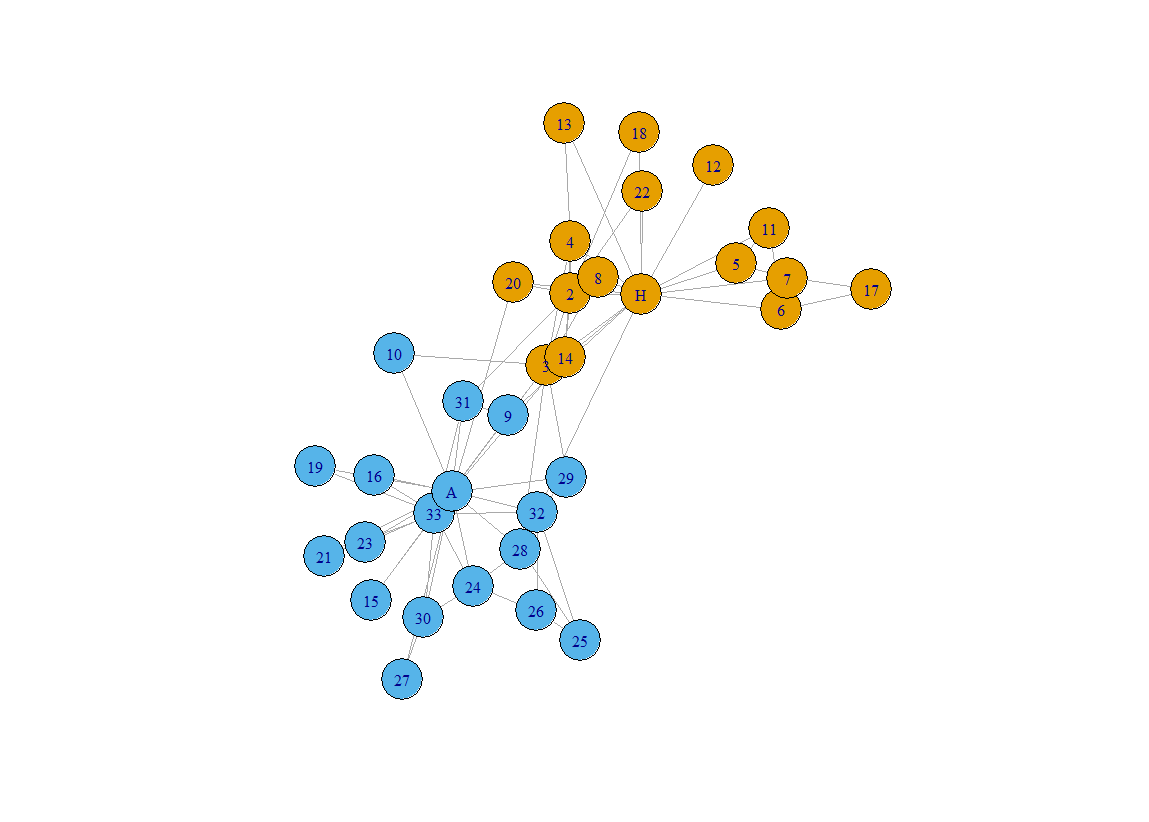
\includegraphics[keepaspectratio]{./images/karate_network.png}}
\caption{The Zachary karate club network with the true split between
members defined by node colors. John A. and Mr.~Hi are denoted by `J'
and `H', with other members being listed as numbers}
\end{figure}

\begin{Shaded}
\begin{Highlighting}[]
\NormalTok{gn\_karate }\OtherTok{\textless{}{-}}\NormalTok{ karate }\SpecialCharTok{|\textgreater{}}
\NormalTok{  igraph}\SpecialCharTok{::}\FunctionTok{cluster\_edge\_betweenness}\NormalTok{()}

\NormalTok{louvain\_karate }\OtherTok{\textless{}{-}}\NormalTok{ karate }\SpecialCharTok{|\textgreater{}}
\NormalTok{  igraph}\SpecialCharTok{::}\FunctionTok{cluster\_louvain}\NormalTok{()}

\NormalTok{sp\_karate }\OtherTok{\textless{}{-}}\NormalTok{ karate }\SpecialCharTok{|\textgreater{}}
\NormalTok{  ig.degree.betweenness}\SpecialCharTok{::}\FunctionTok{cluster\_degree\_betweenness}\NormalTok{()}

\FunctionTok{par}\NormalTok{(}\AttributeTok{mfrow=} \FunctionTok{c}\NormalTok{(}\DecValTok{1}\NormalTok{,}\DecValTok{3}\NormalTok{),}\AttributeTok{mar=}\FunctionTok{c}\NormalTok{(}\DecValTok{0}\NormalTok{,}\DecValTok{0}\NormalTok{,}\DecValTok{0}\NormalTok{,}\DecValTok{0}\NormalTok{)}\SpecialCharTok{+}\DecValTok{1}\NormalTok{)}

\FunctionTok{plot}\NormalTok{(}
\NormalTok{  gn\_karate,}
\NormalTok{  karate,}
  \AttributeTok{main =} \StringTok{"(a)"}
\NormalTok{  )}

\FunctionTok{plot}\NormalTok{(}
\NormalTok{  louvain\_karate,}
\NormalTok{  karate,}
  \AttributeTok{main =} \StringTok{"(b)"}
\NormalTok{)}

\FunctionTok{plot}\NormalTok{(}
\NormalTok{  sp\_karate,}
\NormalTok{  karate,}
  \AttributeTok{main =} \StringTok{"(c)"}
\NormalTok{)}
\end{Highlighting}
\end{Shaded}

\begin{figure}
\centering
\pandocbounded{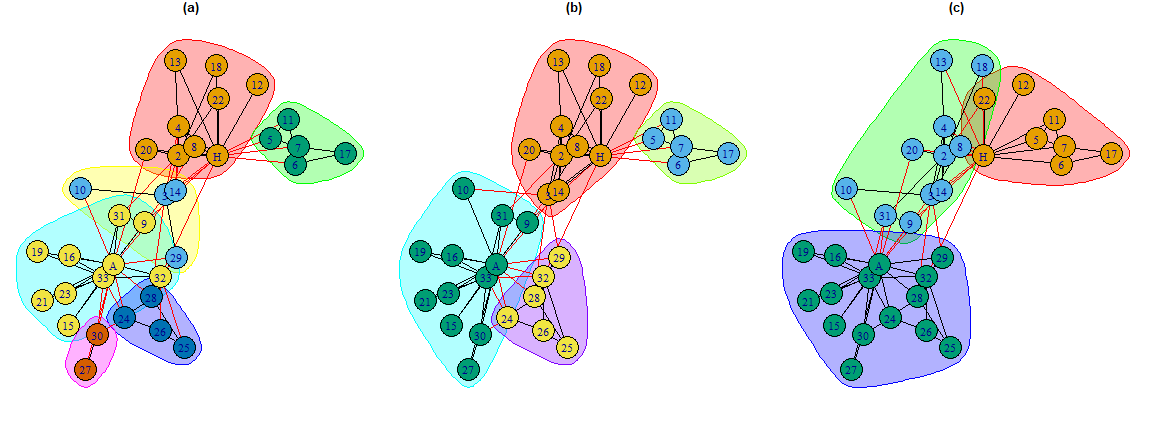
\includegraphics[keepaspectratio]{./images/algorithm_comparison_karate.png}}
\caption{Unsupervised Community Detection by (a) Girvan-Newman, (b)
Louvain and (c) Smith-Pittman for the karate network.}
\end{figure}

\subsection{Other Utility Functions}\label{other-utility-functions}

\subsubsection{Preparing Unlabeled
Graphs}\label{preparing-unlabeled-graphs}

\begin{Shaded}
\begin{Highlighting}[]
\CommentTok{\# Set parameters}
\NormalTok{num\_nodes }\OtherTok{\textless{}{-}} \DecValTok{15}    \CommentTok{\# Number of nodes (adjust as needed)}
\NormalTok{initial\_edges }\OtherTok{\textless{}{-}} \DecValTok{1}   \CommentTok{\# Starting edges for preferential attachment}

\CommentTok{\# Create a directed, scale{-}free network using the Barabási{-}Albert model}
\NormalTok{g }\OtherTok{\textless{}{-}}\NormalTok{ igraph}\SpecialCharTok{::}\FunctionTok{sample\_pa}\NormalTok{(}\AttributeTok{n =}\NormalTok{ num\_nodes, }\AttributeTok{m =}\NormalTok{ initial\_edges, }\AttributeTok{directed =} \ConstantTok{TRUE}\NormalTok{)}

\CommentTok{\# Introduce additional edges to high{-}degree nodes to accentuate popularity differences}
\NormalTok{num\_extra\_edges }\OtherTok{\textless{}{-}} \DecValTok{350}   \CommentTok{\# Additional edges to create more popular nodes}
\FunctionTok{set.seed}\NormalTok{(}\DecValTok{123}\NormalTok{)           }\CommentTok{\# For reproducibility}

\ControlFlowTok{for}\NormalTok{ (i }\ControlFlowTok{in} \DecValTok{1}\SpecialCharTok{:}\NormalTok{num\_extra\_edges) \{}
  \CommentTok{\# Sample nodes with probability proportional to their degree (to reinforce popularity)}
\NormalTok{  from }\OtherTok{\textless{}{-}} \FunctionTok{sample}\NormalTok{( igraph}\SpecialCharTok{::}\FunctionTok{V}\NormalTok{(g), }\DecValTok{1}\NormalTok{, }\AttributeTok{prob =}\NormalTok{  igraph}\SpecialCharTok{::}\FunctionTok{degree}\NormalTok{(g, }\AttributeTok{mode =} \StringTok{"in"}\NormalTok{) }\SpecialCharTok{+} \DecValTok{1}\NormalTok{)  }\CommentTok{\# +1 to avoid zero probabilities}
\NormalTok{  to }\OtherTok{\textless{}{-}} \FunctionTok{sample}\NormalTok{( igraph}\SpecialCharTok{::}\FunctionTok{V}\NormalTok{(g), }\DecValTok{1}\NormalTok{)}

  \CommentTok{\# Ensure we don\textquotesingle{}t add the same edge repeatedly unless intended, allowing self{-}loops}
\NormalTok{  g }\OtherTok{\textless{}{-}}\NormalTok{  igraph}\SpecialCharTok{::}\FunctionTok{add\_edges}\NormalTok{(g, }\FunctionTok{c}\NormalTok{(from, to))}
\NormalTok{\}}

\CommentTok{\# Add self{-}loops to a subset of nodes}
\NormalTok{num\_self\_loops }\OtherTok{\textless{}{-}} \DecValTok{5}
\ControlFlowTok{for}\NormalTok{ (i }\ControlFlowTok{in} \DecValTok{1}\SpecialCharTok{:}\NormalTok{num\_self\_loops) \{}
\NormalTok{  node }\OtherTok{\textless{}{-}} \FunctionTok{sample}\NormalTok{( igraph}\SpecialCharTok{::}\FunctionTok{V}\NormalTok{(g), }\DecValTok{1}\NormalTok{)}
\NormalTok{  g }\OtherTok{\textless{}{-}}\NormalTok{  igraph}\SpecialCharTok{::}\FunctionTok{add\_edges}\NormalTok{(g, }\FunctionTok{c}\NormalTok{(node, node))}
\NormalTok{\}}

\NormalTok{g}
\end{Highlighting}
\end{Shaded}

\begin{verbatim}
## IGRAPH 3a71024 D--- 15 369 -- Barabasi graph
## + attr: name (g/c), power (g/n), m (g/n), zero.appeal (g/n), algorithm
## | (g/c)
## + edges from 3a71024:
##  [1]  2-> 1  3-> 2  4-> 1  5-> 1  6-> 3  7-> 1  8-> 3  9-> 2 10-> 1 11-> 8
## [11] 12-> 1 13->11 14-> 1 15-> 3  3->15  2->14  9->10 10-> 6  6-> 5  9->14
## [21]  8-> 9  1->11  3-> 5 14->11  8->12 15-> 9  2-> 3 14->10  3->10 13->14
## [31]  2-> 4  1-> 1 15-> 7 10->12  1->10 10-> 7  1-> 9 11-> 7 15->12 11-> 7
## [41]  1->11  3-> 6  6-> 2 10-> 5  1->12  7->13  7-> 1  2->11  7-> 6  6->15
## [51]  1->15 11->12  6-> 4 11-> 6 10-> 8  1-> 6 13->15  2-> 1  1-> 2 12-> 2
## [61]  6->13  5-> 6 12-> 3  7-> 4 11-> 9 12->14  4-> 7  2-> 8  4->14  1->15
## + ... omitted several edges
\end{verbatim}

\begin{Shaded}
\begin{Highlighting}[]
\NormalTok{igraph}\SpecialCharTok{::}\FunctionTok{vertex.attributes}\NormalTok{(g)}\SpecialCharTok{$}\NormalTok{name}
\end{Highlighting}
\end{Shaded}

\begin{verbatim}
## NULL
\end{verbatim}

\begin{Shaded}
\begin{Highlighting}[]
\NormalTok{g\_ }\OtherTok{\textless{}{-}}\NormalTok{ ig.degree.betweenness}\SpecialCharTok{::}\FunctionTok{prep\_unlabeled\_graph}\NormalTok{(g)}

\NormalTok{igraph}\SpecialCharTok{::}\FunctionTok{vertex.attributes}\NormalTok{(g\_)}\SpecialCharTok{$}\NormalTok{name}
\end{Highlighting}
\end{Shaded}

\begin{verbatim}
##  [1]  1  2  3  4  5  6  7  8  9 10 11 12 13 14 15
\end{verbatim}

\subsubsection{Plotting Simplified
Edgeplots}\label{plotting-simplified-edgeplots}

\begin{Shaded}
\begin{Highlighting}[]
\FunctionTok{plot}\NormalTok{(}
\NormalTok{  g\_,}
  \AttributeTok{edge.arrow.size =} \FloatTok{0.2}\NormalTok{,}
  \AttributeTok{main =} \StringTok{"Default Network"}
\NormalTok{  )}
\end{Highlighting}
\end{Shaded}

\pandocbounded{\includegraphics[keepaspectratio]{paper_files/figure-latex/unnamed-chunk-3-1.pdf}}

\begin{Shaded}
\begin{Highlighting}[]
\NormalTok{ig.degree.betweenness}\SpecialCharTok{::}\FunctionTok{plot\_simplified\_edgeplot}\NormalTok{(}
\NormalTok{  g\_,}
  \AttributeTok{edge.arrow.size =} \FloatTok{0.2}\NormalTok{,}
  \AttributeTok{main =} \StringTok{"Simplified Network"}
\NormalTok{  )}
\end{Highlighting}
\end{Shaded}

\pandocbounded{\includegraphics[keepaspectratio]{paper_files/figure-latex/unnamed-chunk-4-1.pdf}}

\begin{Shaded}
\begin{Highlighting}[]
\FunctionTok{par}\NormalTok{(}\AttributeTok{mfrow =} \FunctionTok{c}\NormalTok{(}\DecValTok{1}\NormalTok{, }\DecValTok{2}\NormalTok{))}

\NormalTok{sp\_communities }\OtherTok{\textless{}{-}}\NormalTok{ ig.degree.betweenness}\SpecialCharTok{::}\FunctionTok{cluster\_degree\_betweenness}\NormalTok{(g\_)}

\FunctionTok{plot}\NormalTok{(sp\_communities,}
\NormalTok{     g\_,}
     \AttributeTok{edge.arrow.size =} \FloatTok{0.2}\NormalTok{,}
     \AttributeTok{main =} \StringTok{"Default Network"}\NormalTok{)}

\NormalTok{ig.degree.betweenness}\SpecialCharTok{::}\FunctionTok{plot\_simplified\_edgeplot}\NormalTok{(}
\NormalTok{  g\_, }
  \AttributeTok{communities =}\NormalTok{ sp\_communities, }
  \AttributeTok{main =} \StringTok{"Simplified Network"}\NormalTok{)}
\end{Highlighting}
\end{Shaded}

\pandocbounded{\includegraphics[keepaspectratio]{paper_files/figure-latex/unnamed-chunk-5-1.pdf}}

\section{Acknowledgements}\label{acknowledgements}

\section*{References}\label{references}
\addcontentsline{toc}{section}{References}

\phantomsection\label{refs}
\begin{CSLReferences}{1}{0}
\bibitem[\citeproctext]{ref-louvain_paper}
Blondel, Vincent D, Jean-Loup Guillaume, Renaud Lambiotte, and Etienne
Lefebvre. 2008. {``Fast Unfolding of Communities in Large Networks.''}
\emph{Journal of Statistical Mechanics Theory and Experiment} 2008 (10):
P10008. \url{https://doi.org/10.1088/1742-5468/2008/10/p10008}.

\bibitem[\citeproctext]{ref-igraph_article}
Csardi, Gabor, and Tamas Nepusz. 2006. {``The Igraph Software Package
for Complex Network Research.''} \emph{InterJournal} Complex Systems:
1695. \url{https://igraph.org}.

\bibitem[\citeproctext]{ref-igraph_software}
Csárdi, Gábor, Tamás Nepusz, Vincent Traag, Szabolcs Horvát, Fabio
Zanini, Daniel Noom, and Kirill Müller. 2024. \emph{{igraph}: Network
Analysis and Visualization in r}.
\url{https://doi.org/10.5281/zenodo.7682609}.

\bibitem[\citeproctext]{ref-Girvan_Newman_2002}
Girvan, M., and M. E. J. Newman. 2002. {``Community Structure in Social
and Biological Networks.''} \emph{Proceedings of the National Academy of
Sciences} 99 (12): 7821--26.
\url{https://doi.org/10.1073/pnas.122653799}.

\bibitem[\citeproctext]{ref-base2022}
R Core Team. 2022. \emph{R: A Language and Environment for Statistical
Computing}. Vienna, Austria: R Foundation for Statistical Computing.
\url{https://www.R-project.org/}.

\bibitem[\citeproctext]{ref-sp_abstract}
Smith, Benjamin, Tyler Pittman, and Wei Xu. 2024. {``Centrality in
Collaboration: Community Detection for Oncology Researchers.''}
\emph{University of Toronto Journal of Public Health} TODO.
\url{https://arxiv.org}.

\end{CSLReferences}

\end{document}
